\chapter{Moderated Network Models}
The goal of this section is to provide an overview of Moderated Network Models (MNMs) along with some examples of how they can be used to analyze psychological data.
I limit the present discussion to \textit{cross-sectional} MNMs, where the objective is to estimate an undirected network from a sample of $n > 1$ subjects measured on $p$ variables at a single time point. Temporal formulations of these models (i.e., MNMs applied to time series data; both in idiographic and multi-subject settings) will be examined in a separate paper. 

Currently, the MNM framework I present here and implement in the \code{modnets} package supports the analysis of both continuous and binary variables, where each type can serve as either a predictor or an outcome. The simplest case, however, is based on the Gaussian Graphical Model (GGM), wherein all outcomes (i.e., nodes in the network) are assumed to be continuous variables with a multivariate normal distribution. An undirected network consisting of all binary variables is commonly referred to as an \textit{Ising Model}, and has been studied at great length in previous work \cite{lauritzen1996graphical,van2014new,marsman2018introduction}. Moreover, Mixed Graphical Models---where outcome variables may be associated with different univariate distributions---have also received treatment within the literature \cite{yang2014mixed,chen2014selection}. Importantly, all of these models can be formulated as MNMs using the same basic approach, although the results will be subject to different interpretations and are not necessarily associated with a normalizable joint distribution \cite{yang2014mixed, haslbeck2018moderated}. In such cases, this precludes us from computing the likelihood of the model when taken as a whole, thereby preventing us from performing global goodness-of-fit analyses along with model comparison tests. Thus, to outline the basic foundation of MNMs here, I focus on the scenario where all outcome variables are assumed to be continuous, Gaussian variables, as these have the most straightforward interpretation along with a normalizable joint distribution. 

I distinguish between two different types of MNMs: (a) the \textit{exogenous} MNM, and (b) the \textit{endogenous} MNM. The qualifier in each case is meant to refer to the nature of the moderator variable(s) included in the model. For an \textit{exogenous} MNM, we essentially treat the moderator variable(s) as covariates in the model; that is, they are not treated as outcomes which are affected by the other variables, and therefore are not represented as nodes in the resulting network. Instead, they are treated as external components of the process or system under investigation. Identification of moderators as exogenous variables should be based on theory, or based on a reasonable assumption that the variable in question is not influenced by the other variables under study (such as ethnicity, experimental condition, gender, etc.). With \textit{endogenous} moderators, however, these variables will be identified as nodes in the network and treated as outcomes in the construction of the model. This latter case will be most useful in exploratory settings, and will be discussed in a separate paper. Thus, in the remainder of this section I will present the foundation for estimating and interpreting MNMs wherein all outcomes are Gaussian variables and there is only one moderator which is treated as an exogenous variable.

\section{Estimation}
The standard way of constructing a GGM is through joint estimation of model parameters via the standardized inverse covariance matrix---i.e., the \textit{partial correlation matrix}. Let $\bX$ be an $n \times p$ matrix, where each column represents a different variable $(j = 1,\ldots,p)$, and each row contains the response vector for a single subject $(i = 1,\ldots,n)$. For the standard GGM, we assume that the response vectors are multivariate normal:
\begin{equation} \label{mvn}
    \bx_i \sim \N(\bmu, \bSigma)\ \forall i\in\{1,\ldots,n\},
\end{equation}
where $\bmu$ is the $p \times 1$ vector of means, and $\bSigma$ is the $p \times p$ variance-covariance matrix. For simplicity, we will also assume that all the variables have been mean-centered, such that $\bmu = \matr{0}$. Thus, our only objective is to estimate the partial correlation matrix $\bOmega$, which is a $p \times p$ symmetric matrix with zeros in the diagonal and partial correlations between each pair of variables in the off-diagonal. This can be obtained by taking the maximum likelihood estimate (MLE) of $\bSigma$ and standardizing its inverse (i.e., the precision matrix), such that
\begin{equation} \label{ggm}
    \hat{\bSigma} = \frac{\bX\tran\bX}{n},\quad\text{and}\quad \hat{\bOmega} = \I - \bDelta \hat{\bSigma}\inv \bDelta,
\end{equation}
where $\I$ is a $p \times p$ identity matrix, and $\bDelta$ is a diagonal scaling matrix with zeros in the off-diagonal and $\diag{\bDelta} = \diag{\hat{\bSigma}\inv}^{-\frac{1}{2}}$. The resulting estimate of $\bOmega$ therefore encodes the conditional dependence structure of the data, and is used to define the undirected network. 

When moderators, covariates, or any higher-order interaction terms are included in the model, however, this approach is no longer possible. Instead, we can use an approach called \textit{nodewise regression} \cite{haslbeck2015mgm,epskamp2018gaussian}. This method is based on a graph-theoretic approach to structure learning called neighborhood selection \cite{meinshausen2006high}, and entails estimating the network structure via a series of univariate regression models. That is, a separate regression model is constructed for each variable represented as a node in the network, and then the coefficients are aggregated across models to define the final network structure.

For example, imagine that we wanted to model the conditional dependence of three random variables: $X_1$, $X_2$, and $X_3$. Taking the nodewise regression approach, we would begin by constructing three separate univariate regressions:
\begin{equation} \label{mod0}
    \begin{split}
        X_1 &= \beta_{10} + \beta_{12} X_2 + \beta_{13} X_3 + \eps_1 \\
        X_2 &= \beta_{20} + \beta_{21} X_1 + \beta_{23} X_3 + \eps_2 \\
        X_3 &= \beta_{30} + \beta_{31} X_1 + \beta_{32} X_2 + \eps_3.
    \end{split}
\end{equation}
Given that the slope parameters represent directed conditional relationships---e.g., in this example, $\beta_{12}$ is the slope predicting $X_1$ from $X_2$ after conditioning on $X_3$---we can combine relevant pairs of coefficients to obtain the \textit{undirected} conditional dependencies (i.e., partial correlations) between variables. For instance, here the partial correlation between $X_1$ and $X_2$ can be defined as $\omega_{1,2} = \sign{\beta_{12}}\sqrt{\beta_{12}\beta_{21}}$. It is important to note that the signs of $\beta_{12}$ and $\beta_{21}$ will always be the same if and only if the two slope parameters are conditioned on the same covariates (e.g., $X_3$ serves as a covariate in both models), and $n > p$ \cite{williams2019nonregularized}. 

While this equivalence holds when exogenous covariates are included as predictors in the nodewise regressions, it no longer holds when interaction terms are included. That is, imagine that we included a potential moderator $Z$ in the current example. We would now have the following equations:
\begin{equation} \label{mod1}
    \begin{split}
        X_1 &= \beta_{10} + (\beta_{12} X_2 + \beta_{13} X_3 + \beta_{1Z} Z) + (\theta_{1,2Z} X_2 Z + \theta_{1,3Z} X_3 Z) + \eps_1 \\
        X_2 &= \beta_{20} + (\beta_{21} X_1 + \beta_{23} X_3 + \beta_{2Z} Z) + (\theta_{2,1Z} X_1 Z + \theta_{2,3Z} X_3 Z) + \eps_2 \\
        X_3 &= \beta_{30} + (\beta_{31} X_1 + \beta_{32} X_2 + \beta_{3Z} Z) + (\theta_{3,1Z} X_1 Z + \theta_{3,2Z} X_2 Z) + \eps_3.
    \end{split}
\end{equation}
Here I use parentheses to separate main effect terms from interaction terms, where parameters associated with main effects are represented by $\beta$ and those associated with interactions are represented by $\theta$---this distinction is purely for notational clarity.

In these cases, we cannot directly aggregate main effect parameters and transform them into partial correlations. However, we can still approximate the conditional dependencies between variables by averaging over relevant pairs of coefficients; this is a common approach taken in the psychological network literature, even when interactions are not included and exact partial correlations could otherwise be computed \cite{haslbeck2015mgm,epskamp2018gaussian}. While this approach seems simple enough, the examples I've provided so far exemplify cases where each nodewise regression is saturated with all possible terms. In practice, however, model selection procedures are often implemented to determine whether or not all terms should be included in the final models. 

For example, perhaps we find that $X_2$ strongly predicts $X_1$, and so we estimate $\beta_{12}$. But, based on theory or some model selection procedure we conclude that the converse is not true (i.e., $X_1$ is not an important predictor of $X_2$), and so opt to exclude $\beta_{21}$ from the final set of models. This means that we implicitly assume $\beta_{21} = 0$. Now we must choose whether to draw an edge between $X_1$ and $X_2$ in the resulting network. It is common to make this decision by employing either the `AND' or `OR' rule: with the `AND' rule, we only draw an edge between $X_1$ and $X_2$ if both $\beta_{12}$ and $\beta_{21}$ are estimated to be non-zero, whereas with the `OR' rule we draw an edge between the two nodes if at least one of the two relevant parameters is non-zero. In the current example, the edge between $X_1$ and $X_2$ would be calculated as $(\beta_{12} + 0)/2$. 

\section{Analyzing Moderated Networks}
It will be helpful to use an example that illustrates the process of analyzing moderated networks. For simplicity, I will use a subset of the \code{msq} dataset from the R package \code{psych} \cite{psych}. The data consist of $n = 3896$ responses to 75 items on the Motivational State Questionnaire, which measures a variety of mood states on scales ranging from $0$ to $3$. While these variables are clearly ordinal rather than continuous, I chose these data because they resemble a common scenario in psychological research. For this example I will only focus on $5$ items from the questionnaire: \textit{hostile}, \textit{lonely}, \textit{nervous}, \textit{sleepy}, and \textit{depressed}. Here, we will treat \textit{depressed} as an exogenous moderator variable, and will investigate whether the relationships among the other $4$ mood states vary across levels of depression. 

\subsection{Visualization}
First, we begin by mean-centering the data. Although given that $0$ is a value on the scales, it could be argued that mean-centering is not necessary in this case. Nevertheless, centering allows us to assess the relationships between variables at their mean levels, and also reduces the correlations between multiplicative terms and their constituents \cite{lance1988residual,brambor2006understanding}. The next step is to fit $4$ nodewise regressions, one for each of the $4$ outcomes: \textit{hostile}, \textit{lonely}, \textit{nervous}, and \textit{sleepy}. Each regression therefore contains $7$ predictors, with $4$ main effects and $3$ interaction terms. Upon aggregating the coefficients we obtain the following plot.

\begin{figure}[htbp]
    \centering
    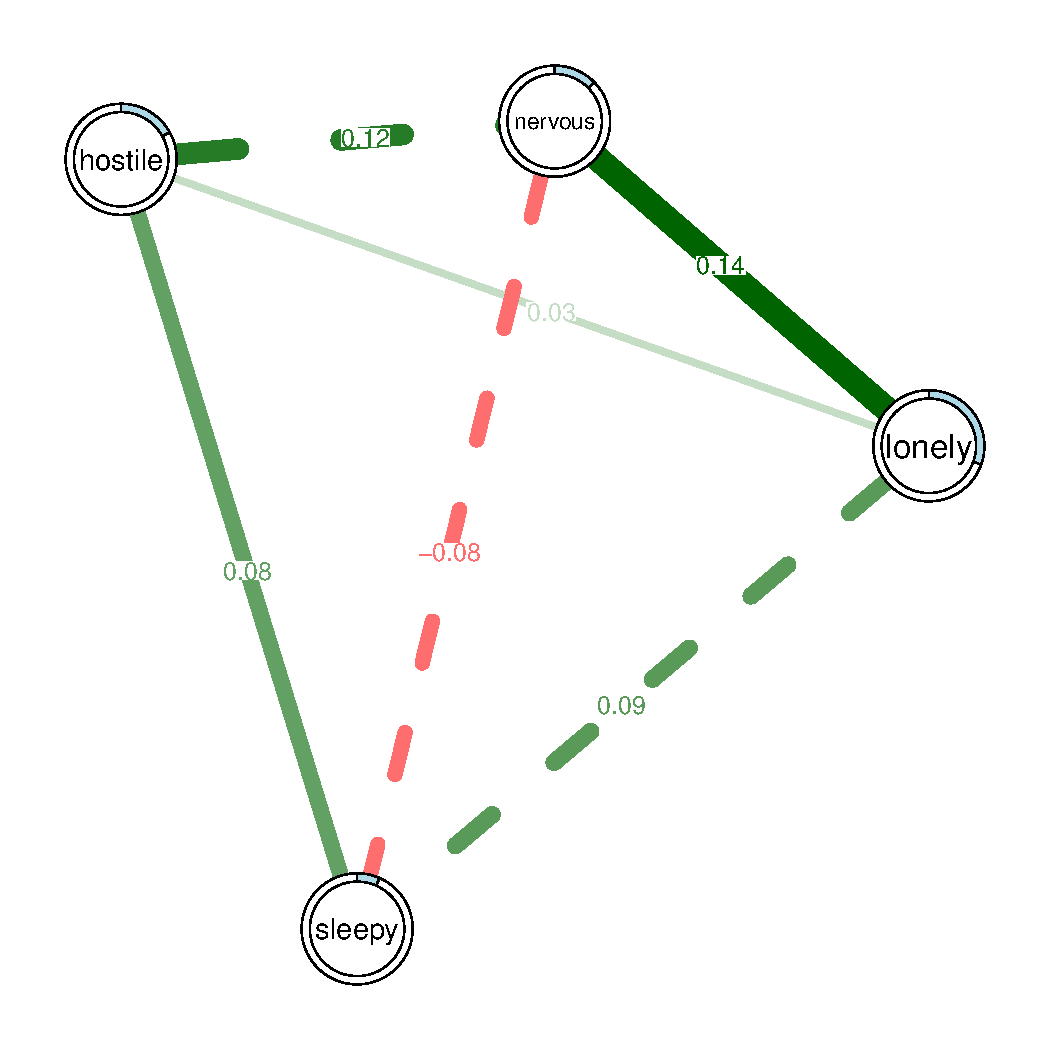
\includegraphics[scale=.6]{images/plot1.pdf}
    \caption{Moderated network model at \textit{depressed} $= 0$, plotted with the AND rule and all interaction terms included in each nodewise regression.}
    \label{fig:plot1}
\end{figure}

In Figure \ref{fig:plot1}, green lines indicate a positive relationship between two variables, red lines indicate negative relationships, and dashed lines indicate that the relationship between two nodes is moderated by the \textit{depressed} variable at $p < .05$. Here the coefficients have been aggregated using the AND rule. Given that all models are saturated, applying either the AND or OR rule produces the same aggregated parameters. However, the rule also determines whether a dashed line is used to indicate the presence of moderation effects---specifically, when using the AND rule I only use a dashed line if \textit{both} relevant interaction terms pass a threshold for significance, while for the OR rule I would draw a dashed line if \textit{at least one} of the two relevant interactions pass the threshold. 

To elaborate, here the interaction term \textit{nervous} $\times$ \textit{depressed} is a significant predictor of \textit{hostile}, and the interaction \textit{hostile} $\times$ \textit{depressed} is a significant predictor of \textit{nervous}. Thus, a dashed line is drawn between the two corresponding nodes in the network. Conversely, the interaction \textit{sleepy} $\times$ \textit{depressed} is a significant predictor of \textit{hostile}, but \textit{hostile} $\times$ \textit{depressed} is not a significant predictor of \textit{sleepy}. So, using the AND rule, the edge between \textit{hostile} and \textit{sleepy} is represented with a solid line, given that only one of the two relevant interaction terms are significant---this edge would be drawn as a dashed line if we chose to apply the OR rule instead. 

\subsection{Visualizing the exogenous moderator}
The \textit{depressed} variable is not represented in the overall network because it is not being considered as an outcome. However, this variable still serves as a predictor in all $4$ regression equations. Thus, we can choose to visualize this variable as an exogenous node in the network as well. In Figure \ref{fig:plot2}, I use a square to represent \textit{depressed} along with arrows denoting its links to the other variables to indicate that this variable only serves as a predictor and is therefore conceptualized as being external to the network. This same approach is taken when other exogenous covariates are included in the model, even if they don't serve as potential moderators.

\begin{figure}[htbp]
    \centering
    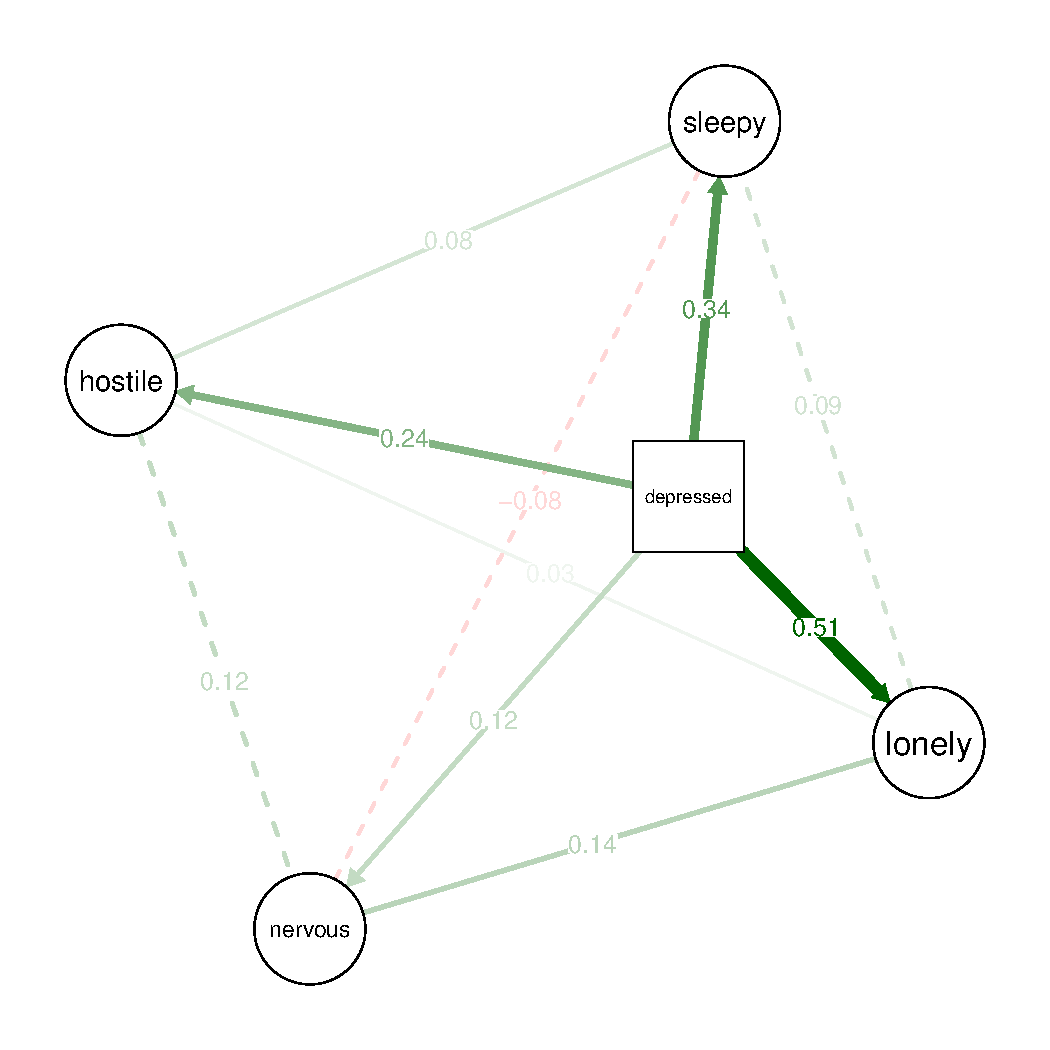
\includegraphics[scale=.6]{images/plot2.pdf}
    \caption{Moderated network model with the exogenous moderator plotted. The color saturation of the edges is scaled against the largest edge weight, which is represented by the beta weight of \textit{depressed} on \textit{lonely}.}
    \label{fig:plot2}
\end{figure}

\subsection{Conditional networks}
Given that there are interaction effects in these models, we cannot interpret the network as representing average or overall conditional dependencies between variables. Instead, these values denote the conditional dependencies between nodes when \textit{depressed} $= 0$; which, since all of the variables have been mean-centered in this example, is equal to the sample mean of \textit{depressed}. The dashed lines in Figures \ref{fig:plot1} \& \ref{fig:plot2} then show us which relationships we should expect to vary across levels of the moderator, while solid lines show us which relationships we should expect to remain constant. Thus it is important to investigate how the network changes across different levels of the moderator, in order to gain more detailed insights into the nature of the interaction effects.

For this example, we will look at how the network changes at increasing levels of depression. That is, using equations \ref{marg} \& \ref{margse} we can compute marginal values of the slope parameters (along with their corresponding standard errors) after conditioning on fixed values of the \textit{depressed} variable (i.e., conditional effects). This is the same approach taken in standard moderation analysis when, given a continuous moderator, researchers often visualize slopes at mean levels of the moderator as well as at $+/-1$ \textit{SD}. Given that the \textit{depressed} variable is positively skewed in this case, however, we will instead compute marginal slopes for the values \textit{depressed} $\in \{0,1,2\}$.

\begin{figure}[htbp]
    \centering
    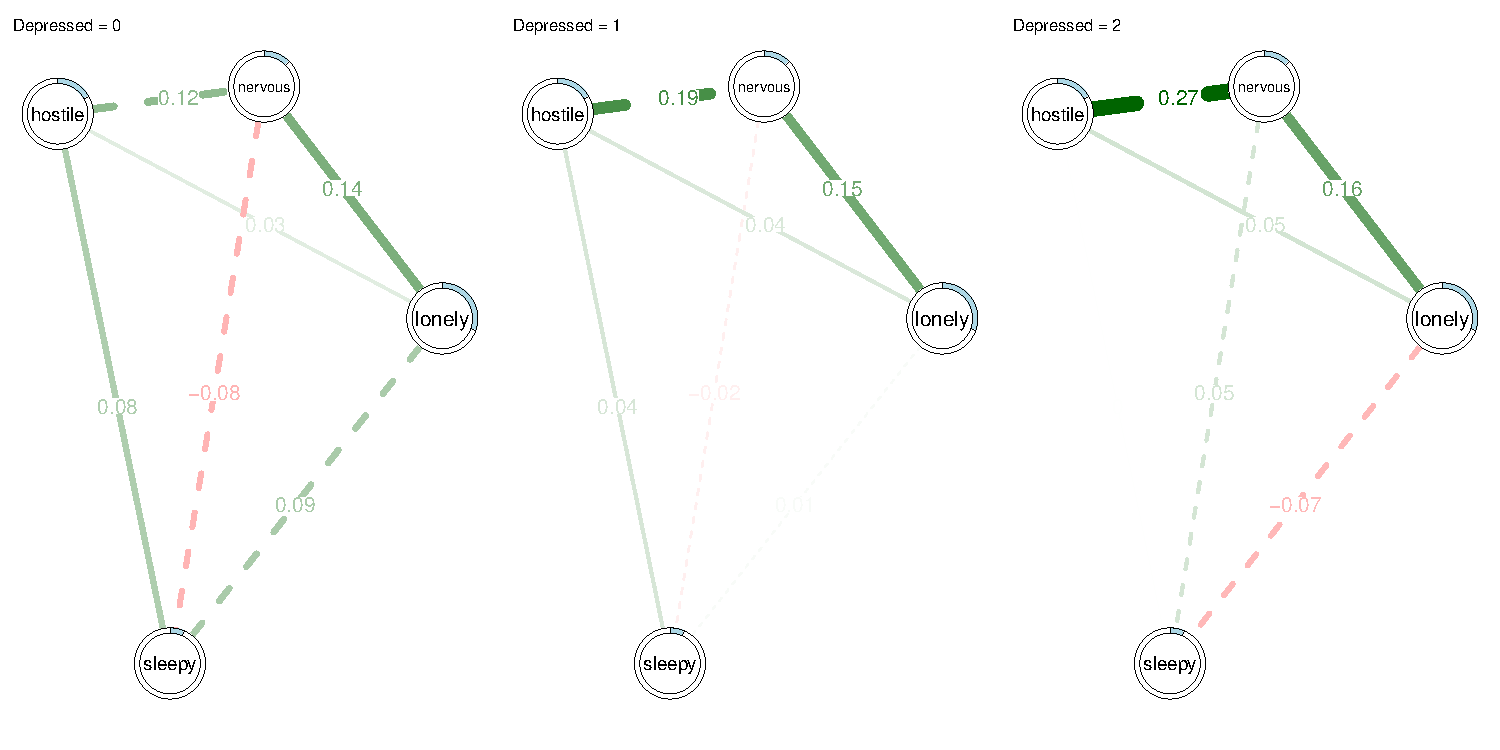
\includegraphics[scale=.6]{images/plot3.pdf}
    \caption{Conditional network models at the values of \textit{depressed} $\in \{0,1,2\}$. Plotted with the AND rule and no significance thresholding.}
    \label{fig:plot3}
\end{figure}

I refer to the plots in Figure \ref{fig:plot3} as \textit{conditional networks} to indicate that they exhibit relationships between variables after conditioning on fixed values of the moderator. In fact, any time we include interaction terms in these models we will always have a conditional network. You'll notice that the first network here is identical to the one previously shown; this is because including interaction terms implicitly means that all constituent main effects represent the slopes when the moderator equals $0$. The only difference between the two visualizations lies in the width and saturation of the edges, as those in the conditional networks plotted in Figure \ref{fig:plot3} are scaled against the largest edge weight, which is the edge connecting \textit{hostile} and \textit{nervous} in the network where \textit{depressed} $= 2$. 

Lastly, while thus far the AND rule has only determined whether or not edges are drawn with a dashed or solid line (based on the presence of significant interaction terms), we can similarly apply the thresholding rule to all model parameters. That is, we can determine whether to draw an edge between two nodes based on whether the main effect terms are significant at some threshold (here, $p < .05$). Using the AND rule, we determine that an edge is drawn between two nodes if both relevant main effects are significant at this cutoff. Thus, in Figure \ref{fig:plot4}, we have a set of networks that only represent the most important relationships between variables, in addition to the most important interaction effects.

\begin{figure}[htbp]
    \centering
    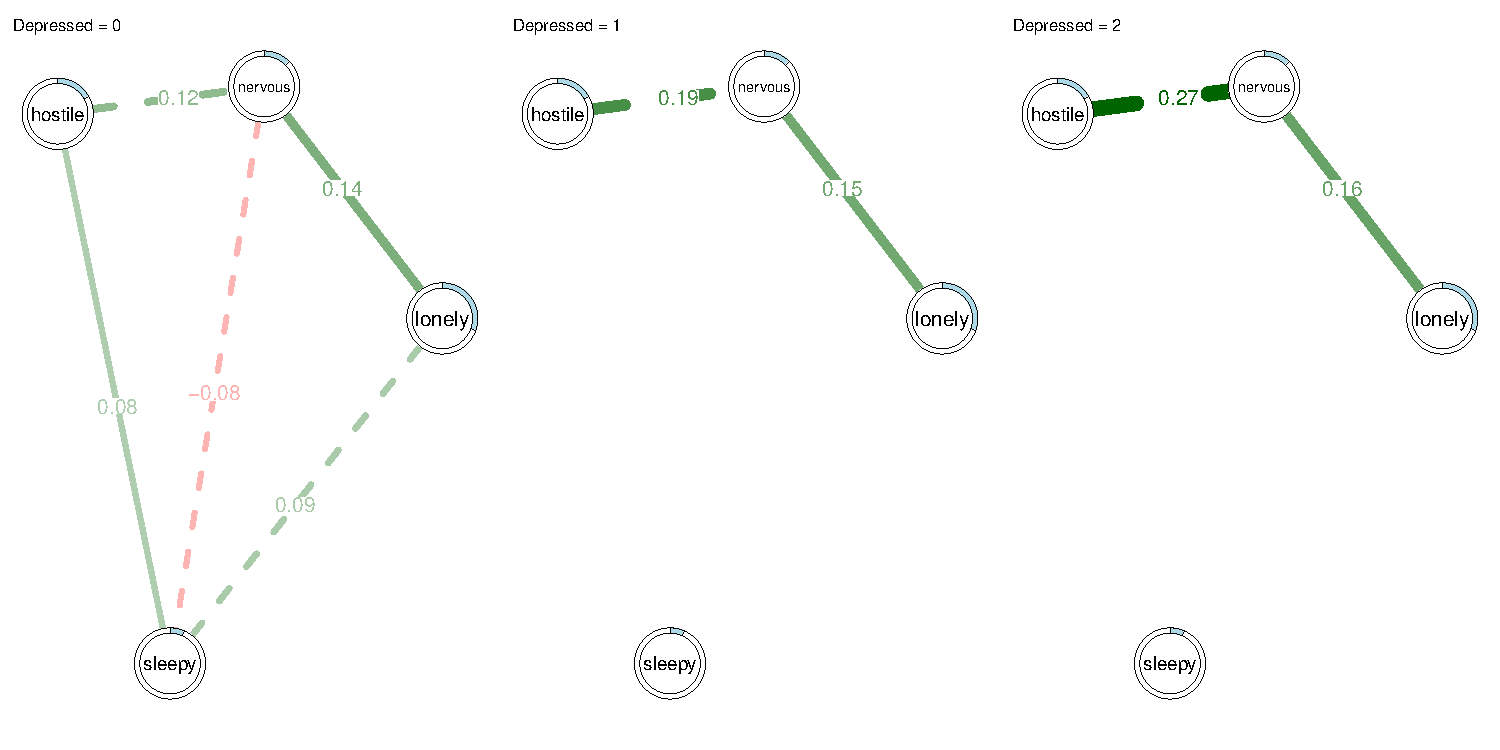
\includegraphics[scale=.6]{images/plot4.pdf}
    \caption{Conditional network models at the values of \textit{depressed} $\in \{0,1,2\}$. Plotted with the AND rule and a significance threshold of $p < .05$.}
    \label{fig:plot4}
\end{figure}

\subsection{Interpreting results}
We can now more clearly see how the network structure changes at increasing levels of depression. Looking only at the plots where thresholding was applied (i.e., Figure \ref{fig:plot4}), we can see that only two relationships persist across levels of depression: (a) that between \textit{nervous} and \textit{hostile}, and (b) between \textit{nervous} and \textit{lonely}. Moreover, we can see that the latter relation remains relatively constant across levels of depression, spanning $\lbrack .14, .16\rbrack$, while the former relation exhibits a significant increase as depression increases, as reflected by the significant interaction effects that modulate the strength of the edge. 

At low levels of depression, we see some other significant, yet small, relationships: (a) a positive relationship between \textit{hostile} and \textit{sleepy}, (b) a positive relationship between \textit{sleepy} and \textit{lonely}, and (c) a negative relationship between \textit{nervous} and \textit{sleepy}. None of these relationships breach our significance threshold at higher levels of depression. The latter two edges appear with dashed lines, however, indicating that they are significantly moderated by levels of depression. We can get a clearer sense of what this means by looking at the non-thresholded set of models in Figure \ref{fig:plot3}. Specifically, both of these relationships switch signs at higher levels of depression, although they do not reach significance in those models. 

If we want to hone-in on any of these results more specifically, we can also look at the marginal changes in the slopes across levels of the moderator, in terms of conditional marginal effects plots. In Figure \ref{fig:conds}, we can clearly see how the relationship between \textit{hostile} and \textit{nervous} increases as depression increases, as well as how the signs of the aforementioned relationships change across this range as well. Lastly, some limitations of this investigation are made clearer in these marginal effects plots. 

\begin{figure}[htbp]
    \centering
    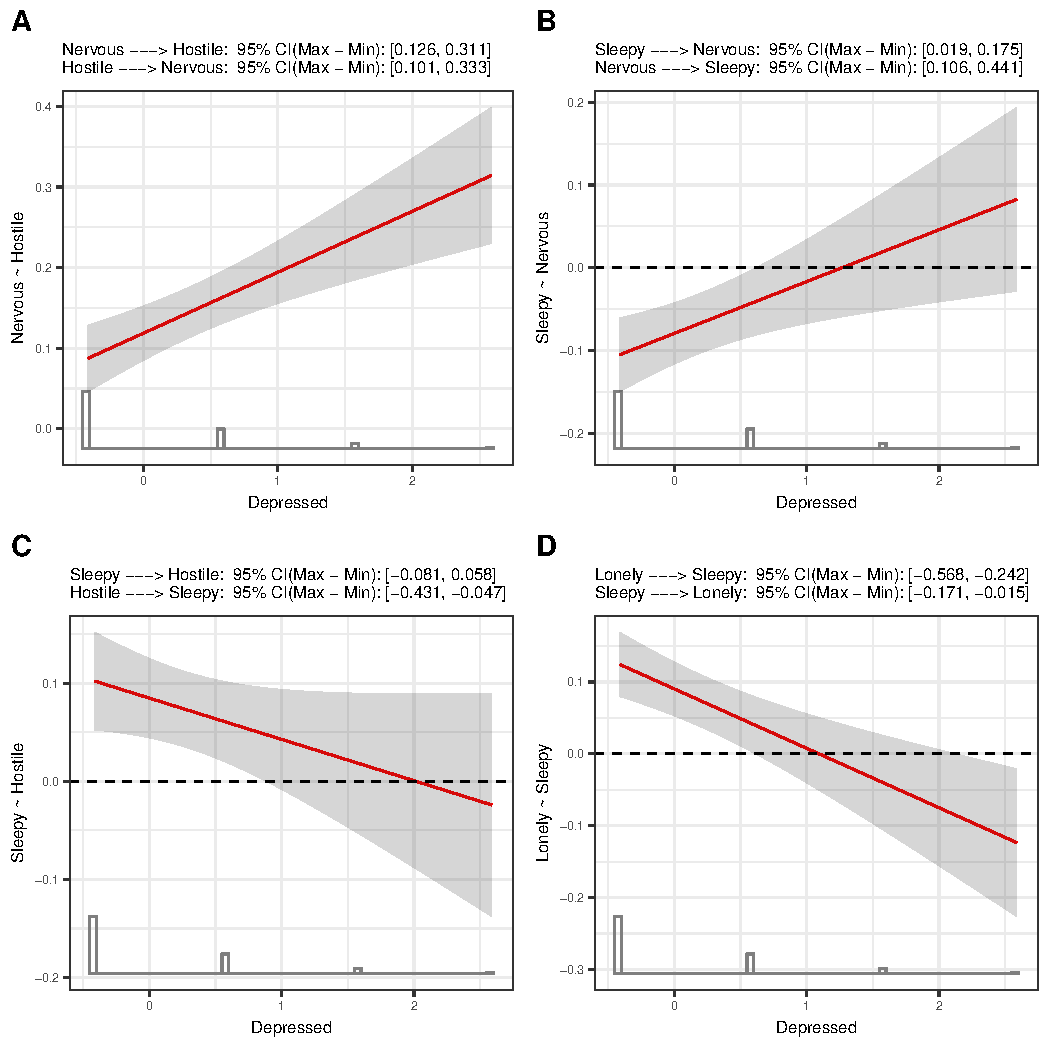
\includegraphics[scale=.7]{images/conds.pdf}
    \caption{Four plots of conditional marginal effects. Each plot represents average values across both relevant interaction terms. In (A), the plot shows the average of two separate conditional marginal effects: that of \textit{hostile} $\times$ \textit{depressed} on \textit{nervous}, as well as for \textit{nervous} $\times$ \textit{depressed} on \textit{hostile}. In (B), the plot shows the average of the conditional marginal effects of \textit{sleepy} $\times$ \textit{depressed} on \textit{nervous}, as well as for \textit{nervous} $\times$ \textit{depressed} on \textit{sleepy}. In (C), the plot shows the average of the conditional marginal effects of \textit{sleepy} $\times$ \textit{depressed} on \textit{hostile}, as well as for \textit{hostile} $\times$ \textit{depressed} on \textit{sleepy}. In (D), this is the average conditional marginal effects of \textit{lonely} $\times$ \textit{depressed} on \textit{sleepy} and \textit{sleepy} $\times$ \textit{depressed} on \textit{lonely}.}
    \label{fig:conds}
\end{figure}

First, the distribution of the \textit{depressed} variable is highly right-skewed; there are a large number of observations at low levels of depression, with fewer and fewer observations as levels of depression increase. Second, the ordinal nature of this variable is made very apparent in the histograms at the base of these plots. Thus, the treatment of this variable as continuous---both in the marginal effects plots and in the analysis---seems somewhat dubious. It would be more appropriate to treat the $4$ possible responses as discrete, ordered categories, at least based on the available sample values. Lastly, the values $\{0,1,2\}$ are not actually represented within the sample once the variable has been mean-centered, and so it would make more sense to plot networks at the values which are used in the analysis. I only chose the three values here for simplicity in this demonstration.

\subsection{Summary}
The goal of this section was to demonstrate a very basic analysis using the moderated network framework. We can see in this example that it is not enough to simply examine one network to understand the conditional dependencies among variables that are subject to interaction effects. Plotting and investigating conditional networks is a crucial part of the analysis, and can reveal patterns in the data that highlight which relationships are most important, which ones change across levels of the moderator, and which relations only emerge under certain conditions (e.g., low values of depression). Continuing with the present example, I will discuss goodness-of-fit indices and model comparison functions that further expand on this type of investigation.

\section{Model Comparison}
Beyond analyzing specific properties of the variables' conditional dependence structure, procedures for model comparison and variable selection (in this case, edge-selection) are important to determine whether or not interaction effects are valuable for the models, as well as whether more parsimonious models with fewer edges can be specified without sacrificing explanatory power. Luckily, when standard estimation procedures are used (as in the current example), standard fit indices and model comparison tests can be employed. There are two levels at which these indices can be assessed: (a) nodewise, and (b) global model fit. 

\subsection{Nodewise Fit Measures}
In the case of models where all outcome variables are assumed to be continuous, we can calculate measures of predictive accuracy for each of the nodewise regressions such as $R^2$, and $R_{adj}^2$ to determine the proportion of the response variance accounted for by the predictors overall, as well as after controlling for the number of predictors (respectively). Additionally, we can assess model fit by computing the log-likelihood, which for a continuous outcome $\bx^{(j)}$ is
\begin{equation}
    \ell(\hat{\bbeta},\hat{\sigma^2}\,|\,\bX) = -\frac{n}{2}\log(2\pi) - \frac{n}{2}\log(\hat{\sigma}^2) - \frac{1}{2\hat{\sigma}^2}\sum_{i=1}^n (x_i^{(j)} - \bx_i^{(-j)}\hat{\bbeta})^2,
\end{equation}
where the superscript $^{(j)}$ indicates the $j$th outcome variable, and $^{(-j)}$ denotes the set of columns from the design matrix (here, $\bX$) that excludes the $j$th variable. The predicted values of $\bx^{(j)}$ are therefore defined as the dot product $\hat{\bx}^{(j)} = \bX^{(-j)}\hat{\bbeta}$, and the MLE for the residual variance is $\hat{\sigma}^2 = \frac{1}{n}\sum_{i=1}^n (x_i^{(j)} - \hat{x}_i^{(j)})^2$. 

Using $\ell(\hat{\bbeta},\hat{\sigma^2}\,|\,\bX)$ we can then compare one model of $j$ (perhaps one including interaction terms) with another by performing a \textit{likelihood ratio test} (LRT), or by computing other fit indices such as the AIC and BIC. These information criteria are defined as
\begin{equation}
    \text{AIC} = 2k - 2\ell(\hat{\bbeta},\hat{\sigma}^2\,|\,\bX),\quad\text{and}\quad\text{BIC} = k\log(n) - 2\ell(\hat{\bbeta},\hat{\sigma^2}\,|\,\bX),
\end{equation}
with $k$ being the number of parameters estimated in the model. The AIC and BIC are transformations of the log-likelihood that afford different emphases in the model selection process by penalizing models with a larger number of parameters. The BIC enforces a stronger penalty than the AIC on models with a greater number of parameters, and is thereby the more conservative of the two \cite{yang2005can}. These criteria are particularly important when we have a large number of variables to consider, or are especially concerned with preserving model fit while limiting ourselves to select a more parsimonious model. 

In the \code{modnets} package, all of these criteria are made available to assess model fit. Nodewise LRTs can be conducted to compare models for each node, individually, across different specifications of the network, and indices of predictive accuracy---namely, $R^2$ and $R_{adj}^2$---can be depicted graphically to accompany the network representations. This approach was first used by \cite{haslbeck2017predictable}, but has been expanded in the \code{modnets} package to allow for model comparison. For instance, in Figure \ref{fig:plot5} we visualize the same model as in Figure \ref{fig:plot1}, but use blue rings around each node in (A) to denote the $R^2$ value of each model in comparison with a model that excludes the interaction terms, as well as the \textit{depressed} variable. Specifically, the light blue represents the $R^2$ of the reduced model (excluding interaction terms and the \textit{depressed}) variable, while the darker blue represents the additional $R_{\Delta}^2$ that is contributed by including \textit{depressed} and the accompanying interaction terms. 

\begin{figure}[htbp]
    \centering
    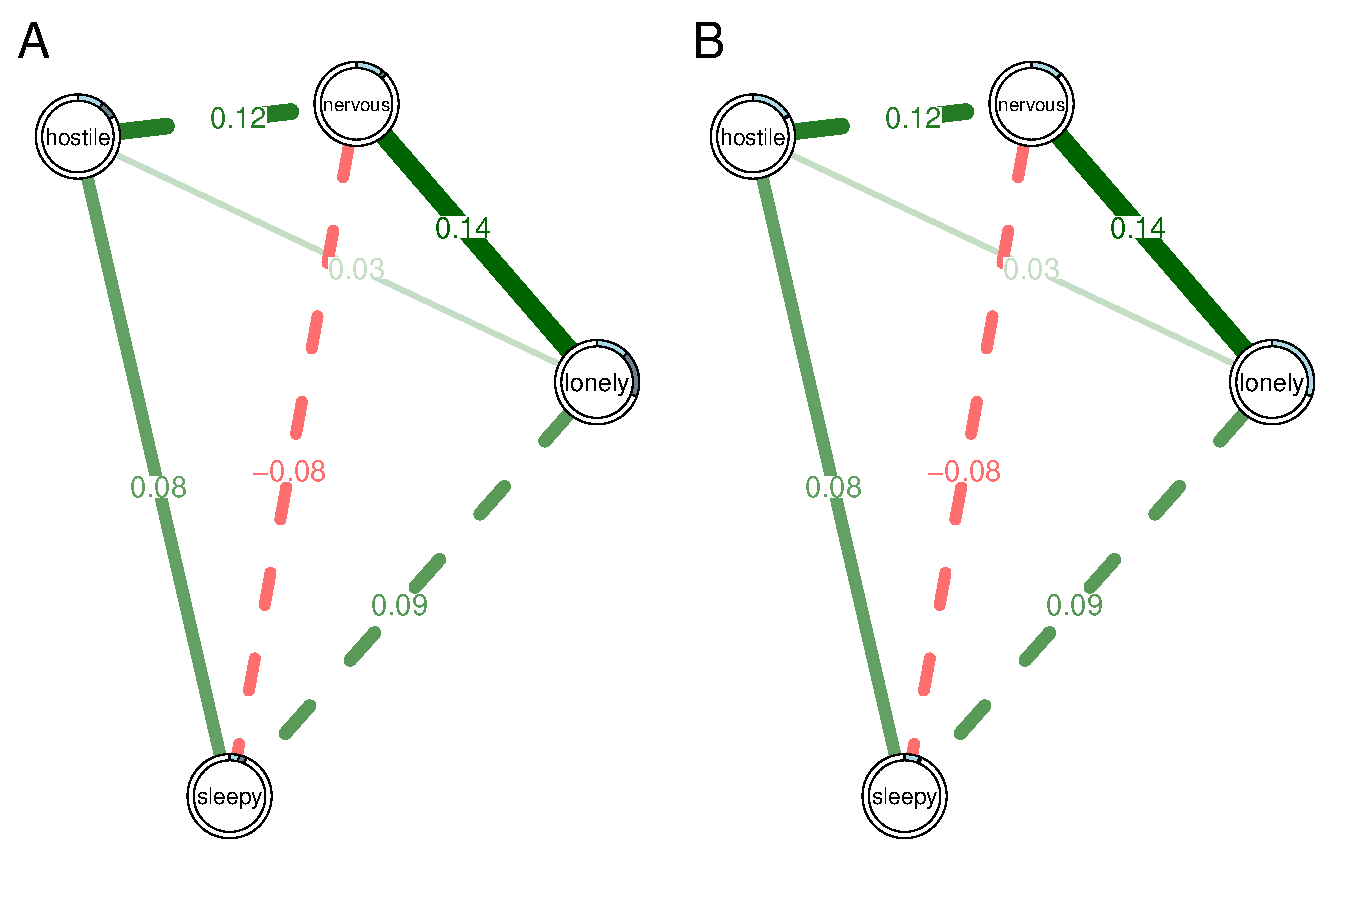
\includegraphics[scale=.6]{images/plot5.pdf}
    \caption{These plots show the same network model as in Figure 2, but with two different comparisons represented by the blue shading in each node. In (A), the light blue shading represents the $R^2$ for each nodewise regression where \textit{depression} is not included in any of the models, while the dark blue shading shows the $R_{\Delta}^2$ given the models including \textit{depression} as well as all of its interaction effects. In (B), the models being compared to the moderation models include \textit{depressed} as a covariate.}
    \label{fig:plot5}
\end{figure}

When we include \textit{depressed} as a covariate, however, we can now see that the increase in $R^2$ after including the interactions is very small (B). This highlights the importance of using fit indices in addition to these metrics in order to determine which model should be interpreted.

\subsection{Global Fit Measures}
It is possible to obtain similar fit measures to describe the fit of all nodewise models taken together. That is, in certain circumstances we can compute the multivariate log-likelihood as well as the corresponding AIC and BIC values to assess global fit across models. This is currently only possible when all outcomes are continuous and assumed to be multivariate normal. However, even this may be undefined in certain cases when many interaction terms are included, particularly when this prevents the residual covariance matrix from being positive definite \cite{yang2014mixed,haslbeck2018moderated}. The multivariate normal log-likelihood can be written as
\begin{equation}
    \ell(\hat{\bX}, \hat{\bSigma}\,|\,\bX) = \sum_{i=1}^n -\frac{m}{2}\log(2\pi) - \frac{1}{2}\log(|\hat{\bSigma}|) - \frac{1}{2}(\bx_i - \hat{\bx}_i)\hat{\bSigma}\inv(\bx_i - \hat{\bx}_i)
\end{equation}
where $m$ is the number of nodewise regression models being estimated (which may be different from $p$, the number of variables, e.g. when the moderator is exogenous), $\hat{\matr{M}}$ is an $n \times m$ matrix containing the predicted values for each nodewise regression, $\hat{\bSigma}$ is the $m \times m$ residual covariance matrix, and $|\hat{\bSigma}|$ is its determinant.

The global AIC and BIC can also be calculated from $\ell(\hat{\matr{M}}, \hat{\bSigma}\,|\,\bX)$, where we supplant $k$ with $k^*$ to denote the number of estimated parameters summed across \textit{all} nodewise models. From here, we can conduct global LRTs and use the other fit indices to compare network models taken as a whole.

In sum, we can use both nodewise fit measures along with global fit measures to optimize information criteria at each level of analysis and select the best model in accordance with our (the researcher's) priorities. In each of these cases, however, I am assuming that there is a clear set of candidate models for us to consider. In the present example, I've presented $3$ clear candidate models: (a) the set of models excluding \textit{depressed}, (b) the set of models including \textit{depressed} as a covariate, and (c) the set of models including \textit{depressed} and its associated interaction terms as covariates. Yet, it may not always be this easy, as we may have many more variables to consider, or may be conducting an even more exploratory analysis wherein the goal is to assess an array of potential moderators and determine the most parsimonious set of models.

\section{General Discussion}
As psychological network models become more widely used across different areas of research, it is clear that methodological extensions are much needed. One recent approach spearheaded by \cite{epskamp2017generalized} has been to integrate network models with latent variable models in an effort to create `hybrid networks' for studying psychological phenomena. Other new approaches have included networks for time-series models, particularly those that apply to multiple subjects sampled over time \cite{hamaker2018frontiers}, as well as those that use non-parametric, time-varying models to accommodate data that violate parametric model assumptions \cite{bringmann2017changing}. The project described in this paper aims to expand on network models in another, complementary way, and that is by extending current approaches to move beyond strictly pairwise relationships and include higher-order effects such as moderators and interaction terms.

\subsection{Extending Pairwise Networks with Temporal Data}
The central focus of this paper has been on incorporating moderation effects in psychological network models. The present paper focuses exclusively on \textit{cross-sectional networks}, wherein the goal is to study relationships between variables sampled from multiple subjects at a single point in time. The \code{modnets} package is explicitly designed to handle other data types as well---particularly idiographic data, where repeated-measures are analyzed from a single individual, and multilevel data, where multiple subjects are repeatedly measured over time. These will be discussed at greater length in another paper, but for now it can at least be said that the foundations of moderated network models also exist for analyzing repeated, ordered observations, and their implementation in the \code{modnets} package will make it the first available software for analyzing and fitting these types of models.
